\section{Crear una cuenta de GitHub}
\begin{itemize}
    \item[\textbf{\texttt{1.-}}] Abrir un navegador web (ej. Google Chrome, Firefox, Brave, Opera, etc.).
    \item[\textbf{\texttt{2.-}}] Buscar "GitHub" en el buscador web o bien, usar la siguiente url ``\textcolor{Naranjap}{https://github.com}''.
    \item[\textbf{\texttt{3.-}}] Dar click en el botón con la leyenda ``Sign Up'' como se muetra en la siguiente imagen.
\end{itemize}
\begin{figure}[H]
    \centering
    
\includegraphics[width=\paperwidth-12cm]{screenshot-rocks-GitHub-cursor.png}
    \caption{Sign Up}
\end{figure}
\begin{itemize}
    \item[\textbf{\texttt{4.-}}] Escribir su correo electrónico en la caja de texto y posteriormente presionar en el botón con la leyenda ``Continue'' como se muestra en la siguiente imagen.
\end{itemize}
\begin{figure}[H]
    \centering
    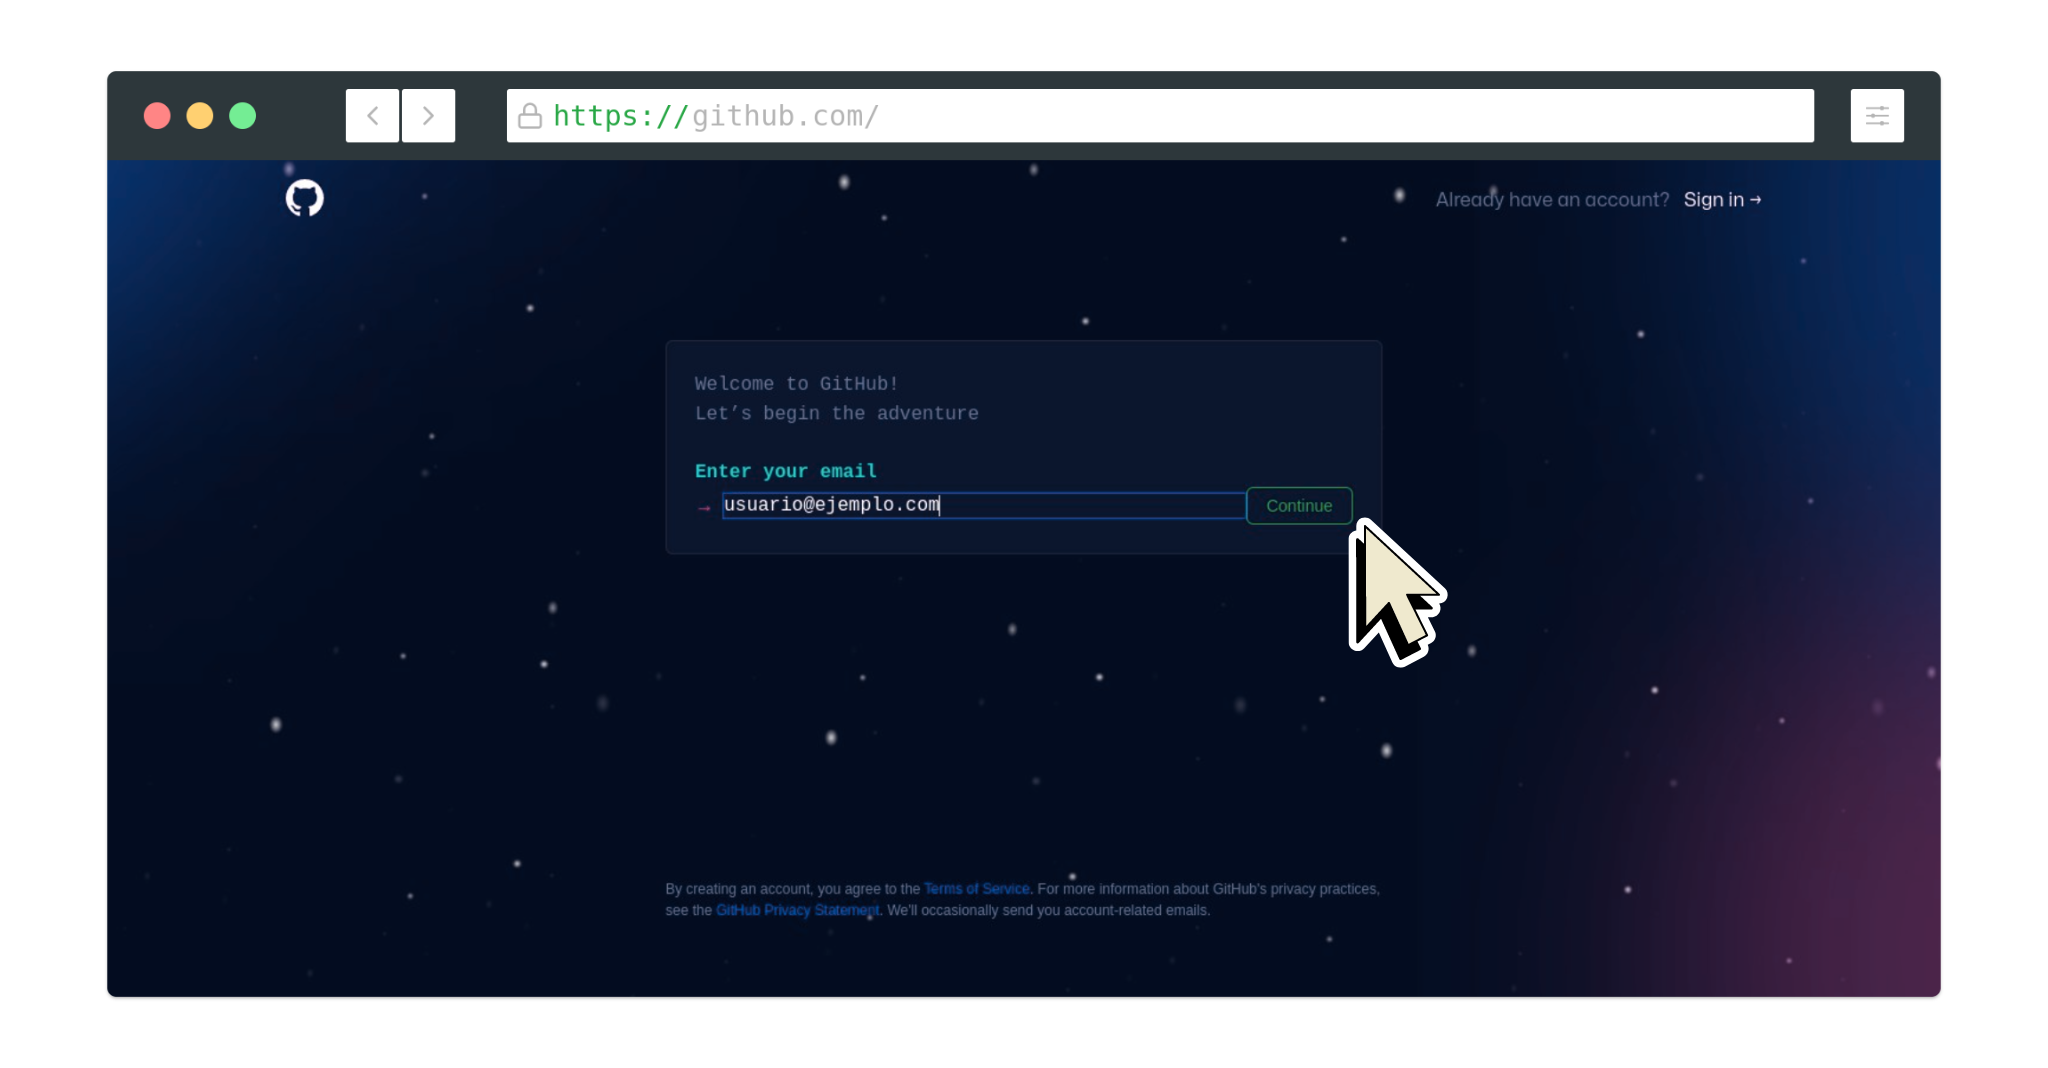
\includegraphics[width=\paperwidth-12cm]{screenshot-rocks-GitHub-SignIn-cursor.png}
    \caption{Ingresar correo electrónico}
\end{figure}
\begin{itemize}
    \item[\textbf{\texttt{5.-}}] Crear una contraseña y escribirla en la caja de texto, finalmente presionar en el botón con la leyenda ``Continue'' como se muestra en la siguiente imagen.
\end{itemize}
\begin{figure}[H]
    \centering
    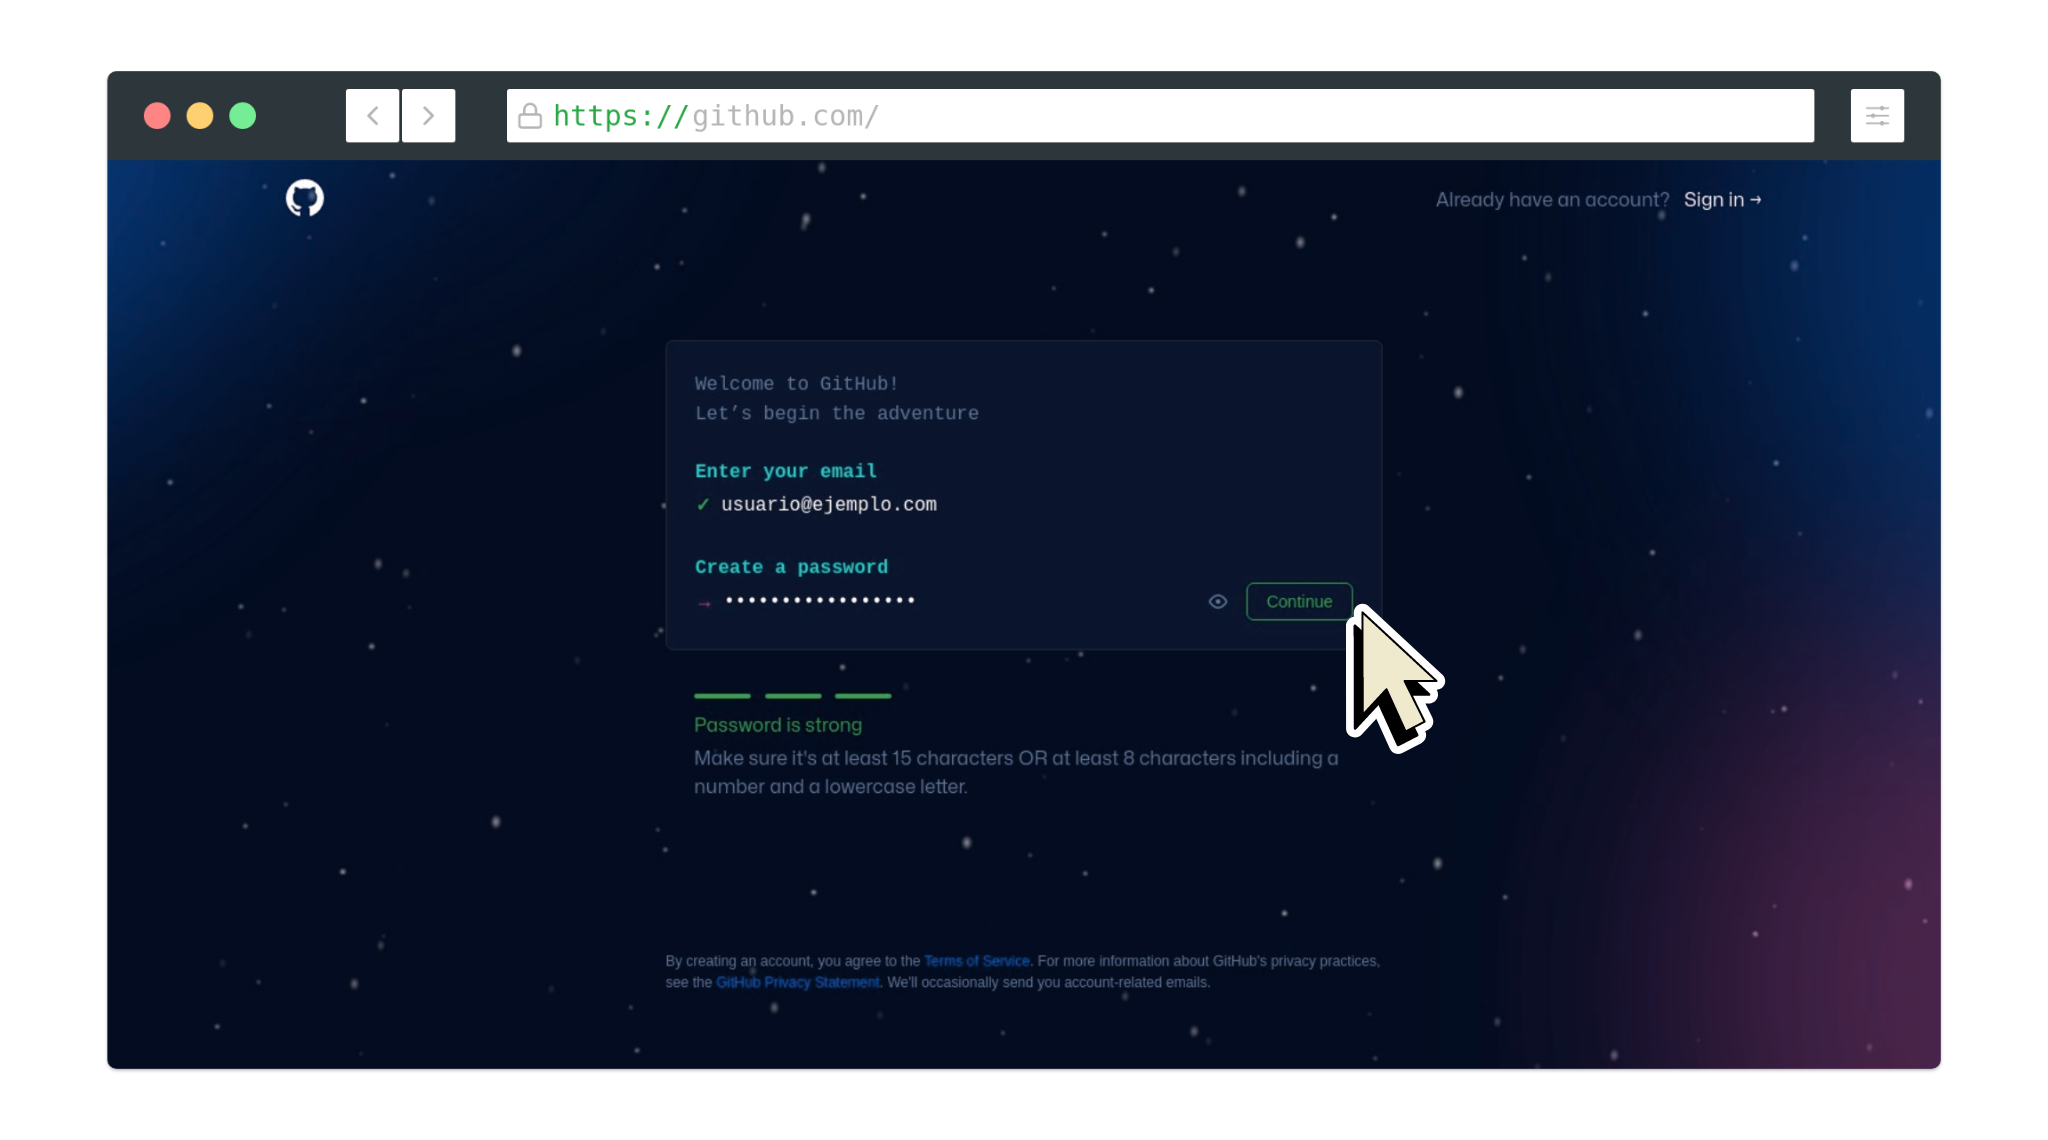
\includegraphics[width=\paperwidth-12cm]{screenshot-rocks-GitHub-Password-cursor.png}
    \caption{Crear contraseña}
\end{figure}
\begin{itemize}
    \item[\textbf{\texttt{6.-}}] Crear un nombre de usuario (solo se permiten caracteres alfanumericos y guiones, no puede iniciar o terminar con un guión) y escribirlo en la caja de texto, después presionar en el botón con la leyenda ``Continue'' como se muestra en la siguiente imagen. Tenga en cuenta que este será el nombre que aparecerá en su perfil.
\end{itemize}
\begin{figure}[H]
    \centering
    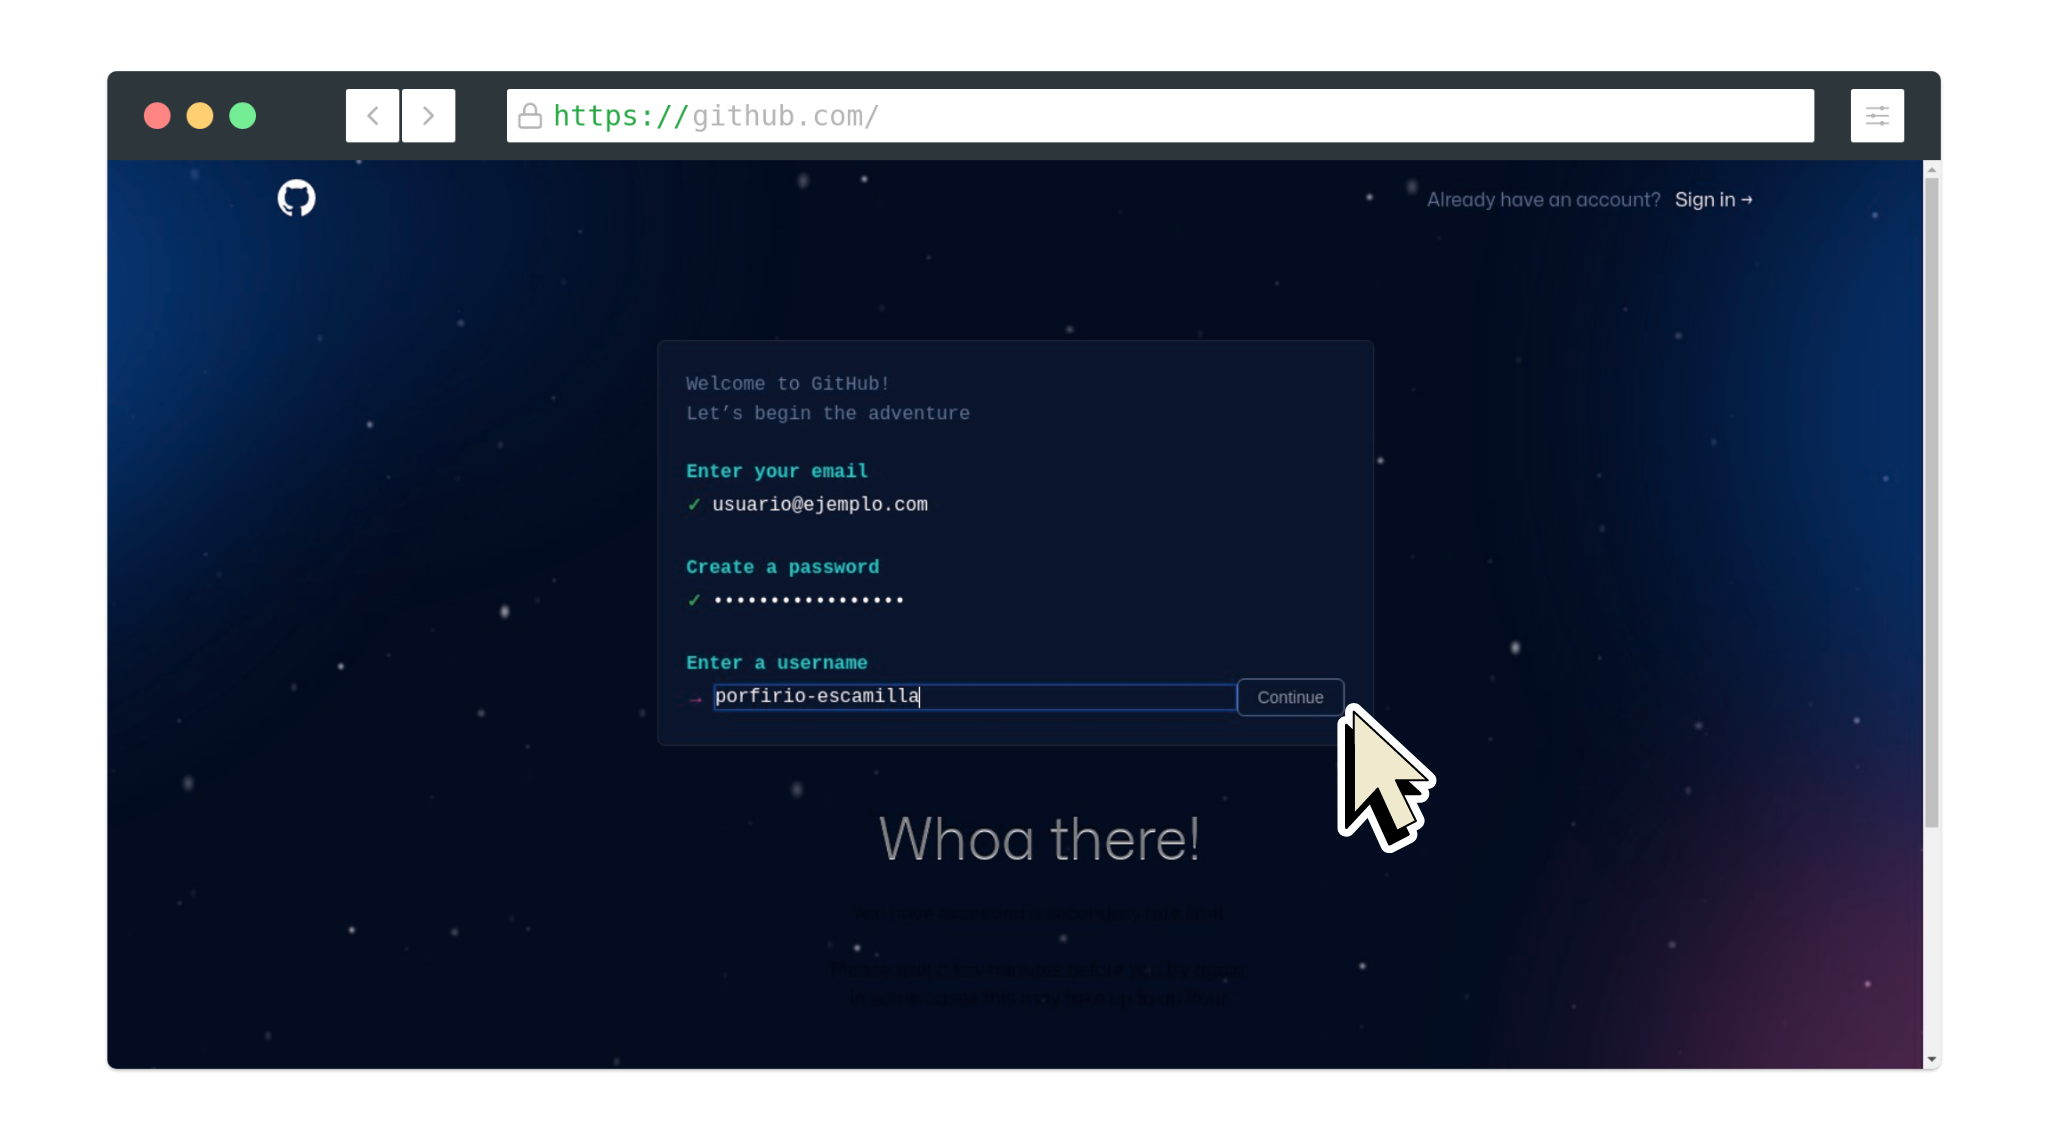
\includegraphics[width=\paperwidth-12cm]{screenshot-rocks-Username-cursor.png}
    \caption{Crear nombre de usuario}
\end{figure}
\begin{itemize}
    \item[\textbf{\texttt{7.-}}] Escribir en la caja de texto una `y' si se quiere recibir anuncios por correo o una `n' en caso contrario, luego presionar en el botón con la leyenda ``Continue'' como se muestra en la siguiente imagen.
\end{itemize}
\begin{figure}[H]
    \centering
    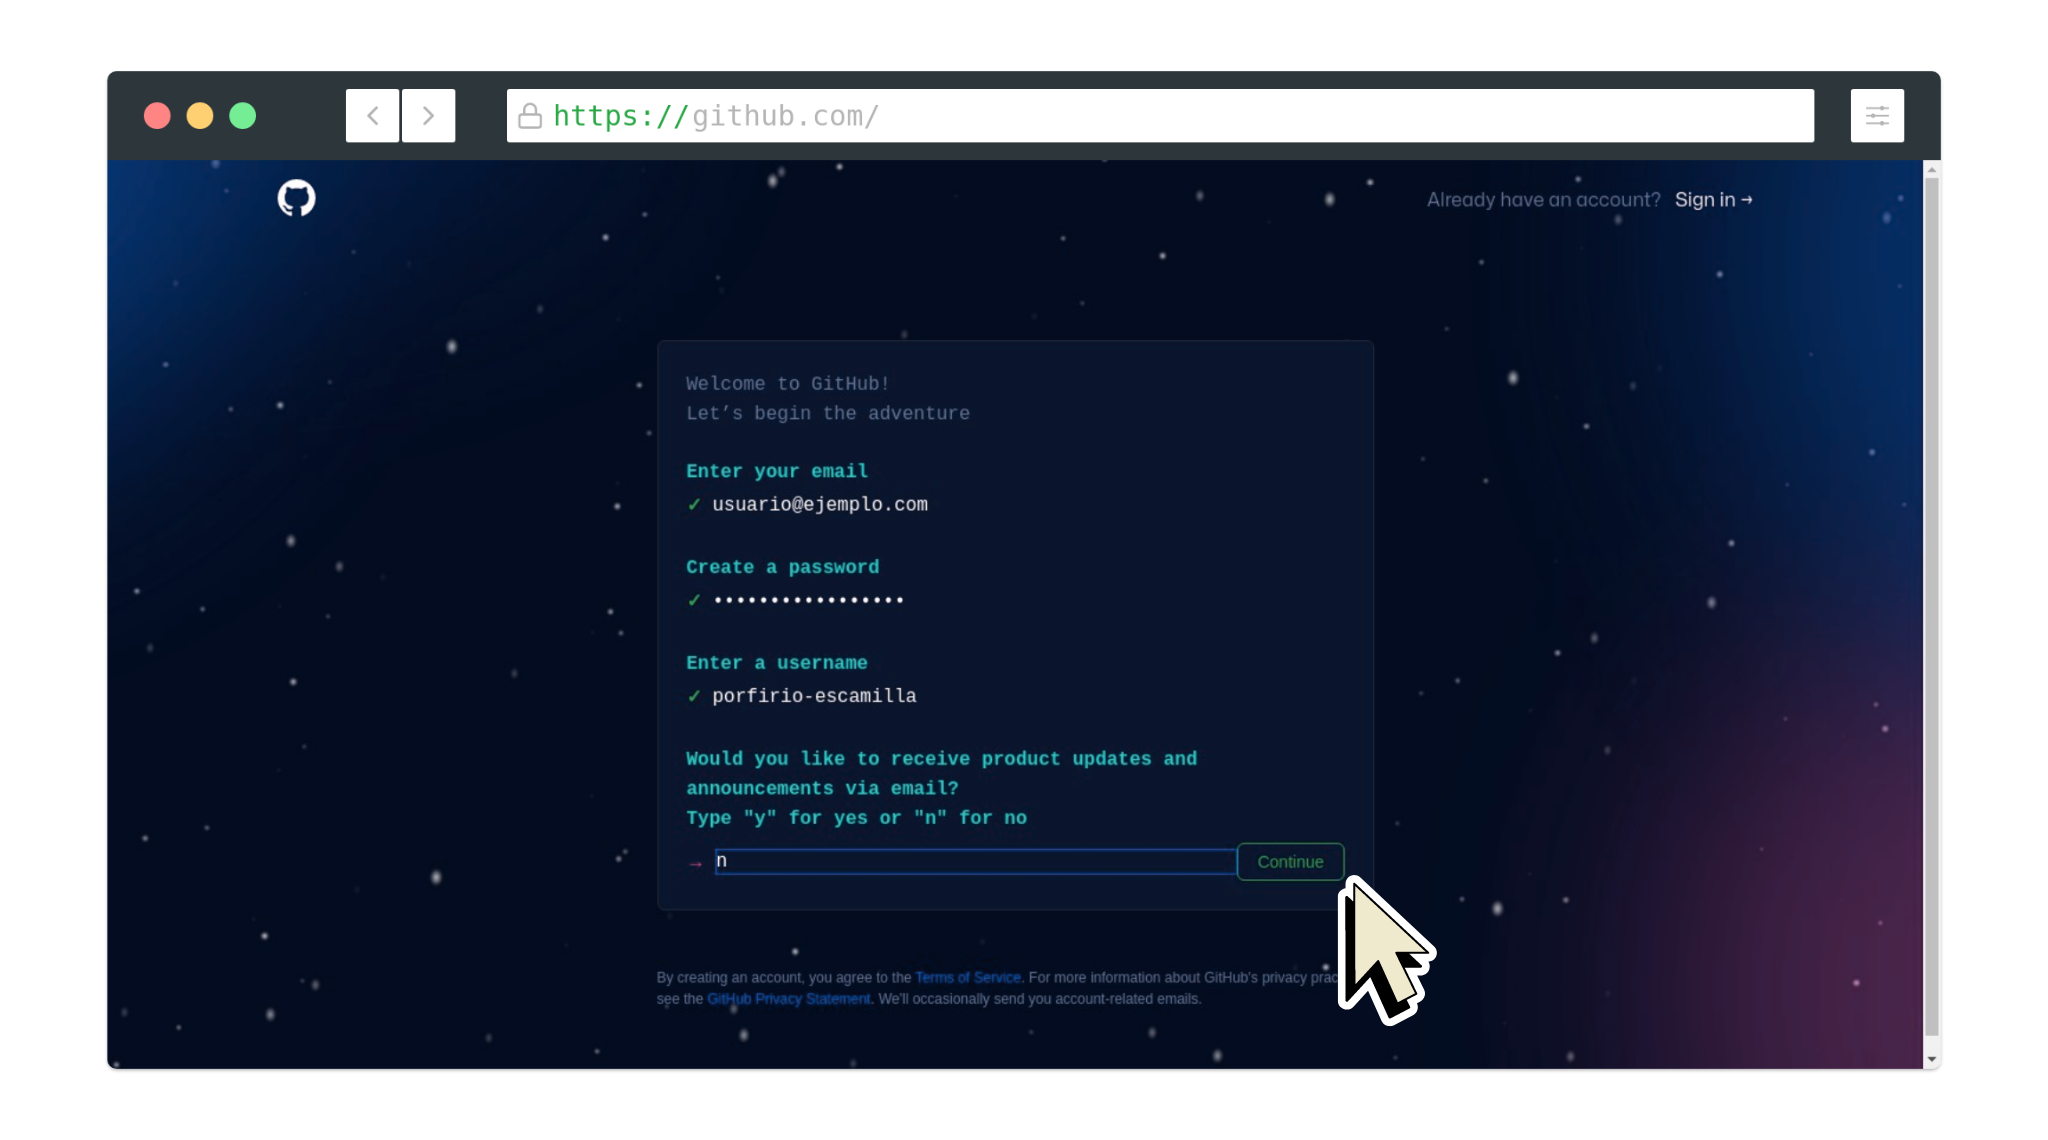
\includegraphics[width=\paperwidth-12cm]{screenshot-rocks-GitHub-Anuncios-cursor.png}
    \caption{Anuncios}
\end{figure}
\begin{itemize}
    \item[\textbf{\texttt{8.-}}] Presionar el botón con la leyenda ``Verificar'' como se muestra en la siguiente imagen.
\end{itemize}
\begin{figure}[H]
    \centering
    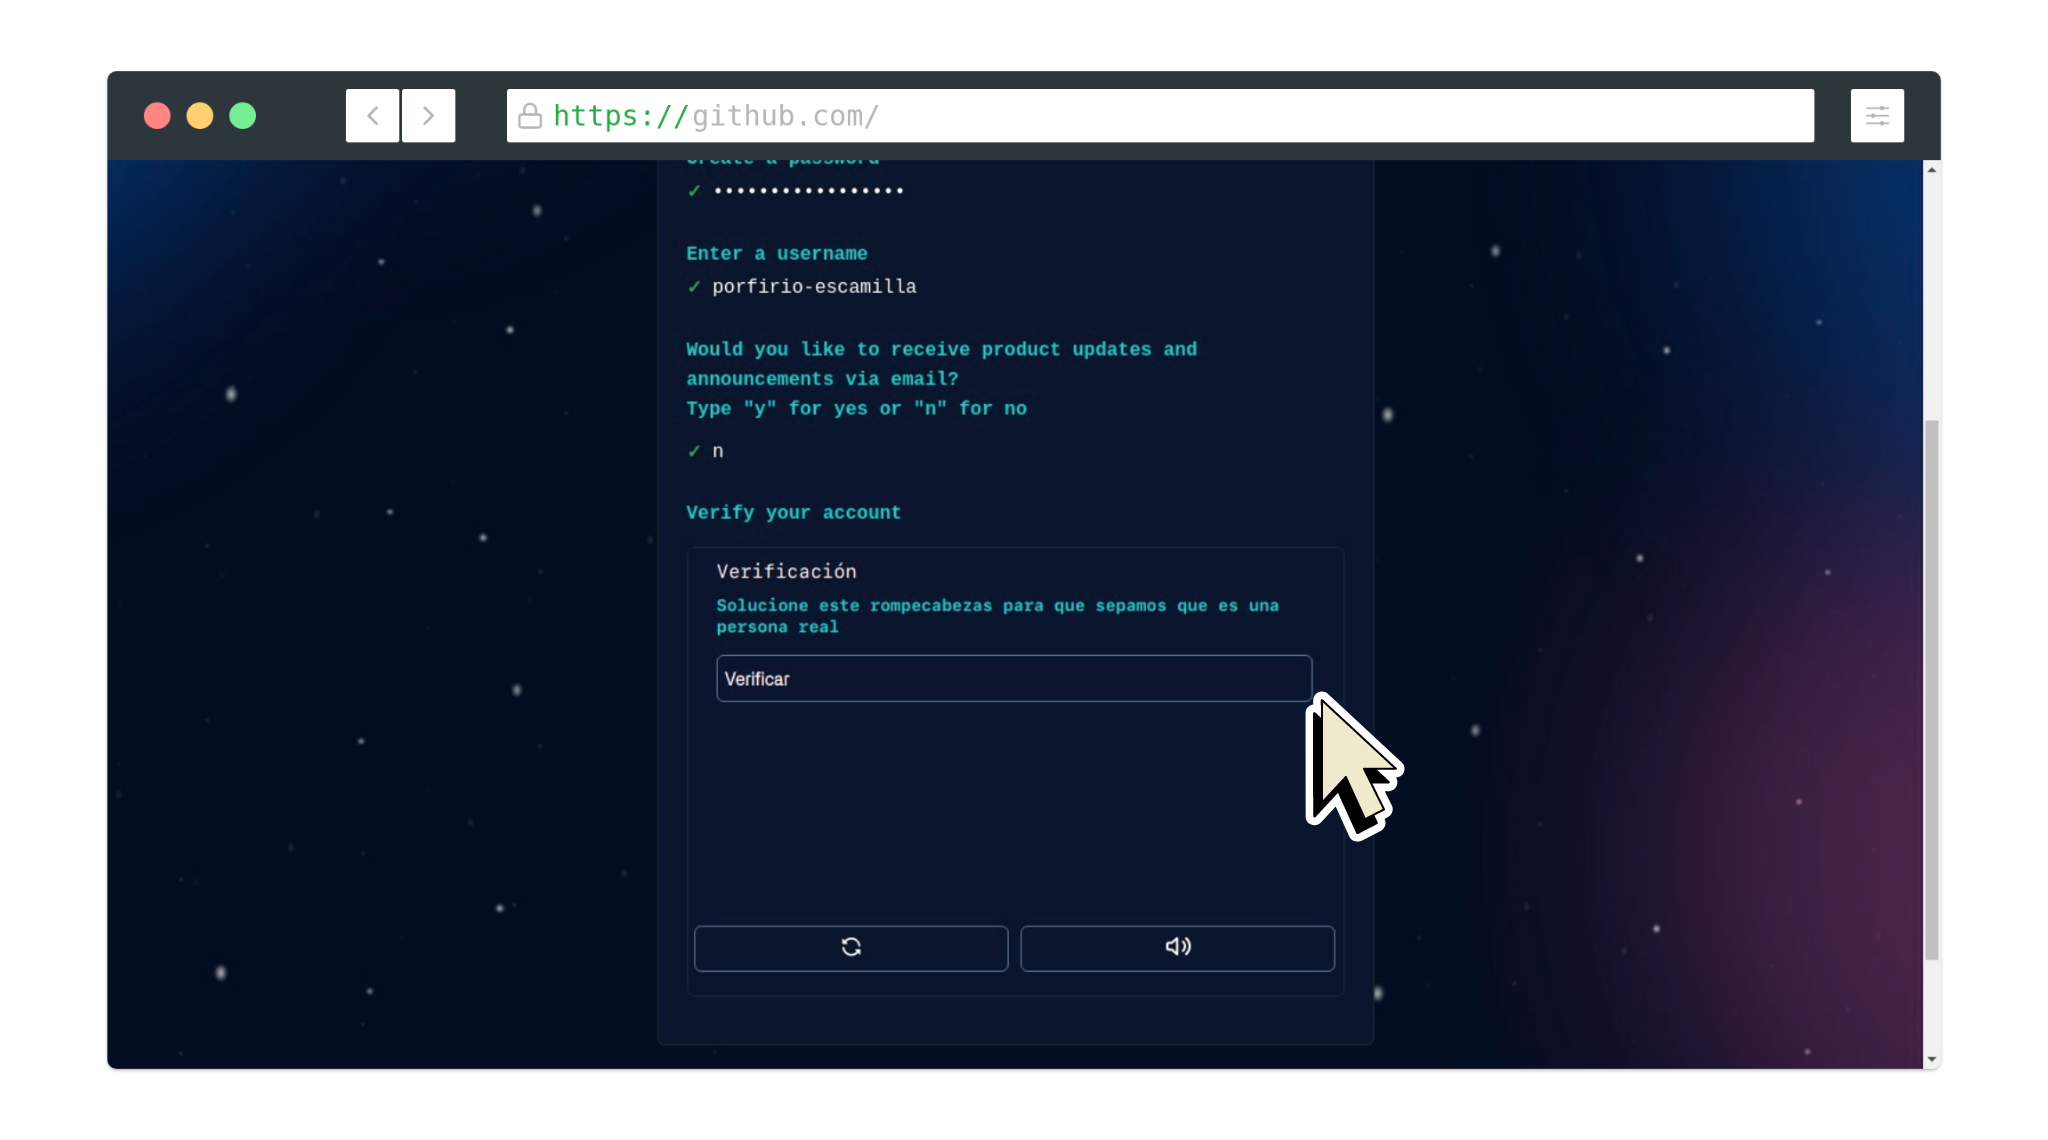
\includegraphics[width=\paperwidth-12cm]{screenshot-rocks-GitHub-Verificacion-cursor.png}
    \caption{Anuncios}
\end{figure}
\begin{itemize}
    \item[\textbf{\texttt{9.-}}] Seguir las instrucciones de GitHub, remarcadas en la siguiente imagen.
\end{itemize}
\begin{figure}[H]
    \centering
    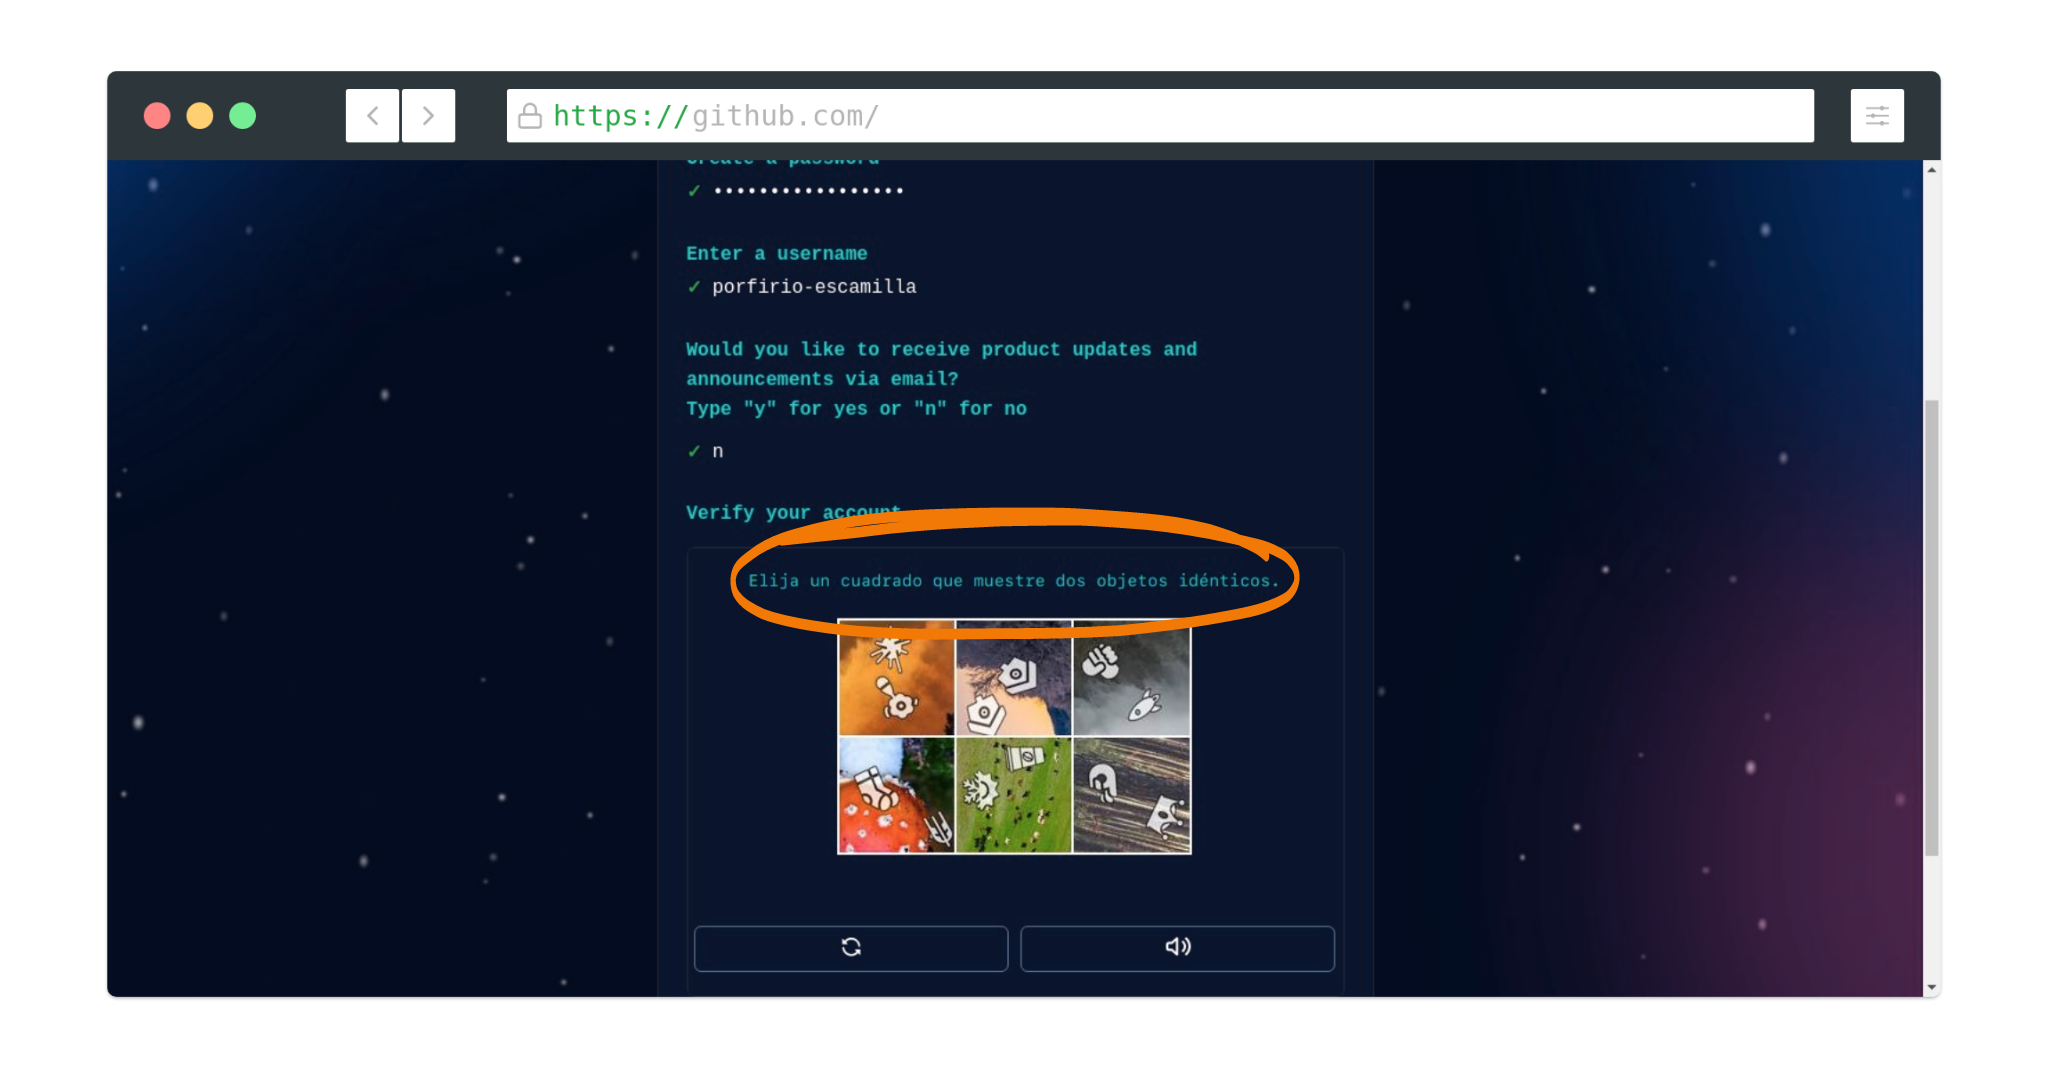
\includegraphics[width=\paperwidth-12cm]{screenshot-rocks-GitHub-Verificacion-Instrucciones-Resalte.png}
    \caption{Anuncios}
\end{figure}